%%%%%%%%%%%%%%%%%%%%%%%%%%%%%%%%%%%%%%%%%%%%%%%%%%%%%%%%%%%%%%%%%%%%%%%%%%%%%%%%
%2345678901234567890123456789012345678901234567890123456789012345678901234567890
%        1         2         3         4         5         6         7         8

\documentclass[letterpaper, 10 pt, conference]{ieeeconf}  % Comment this line out
                                                          % if you need a4paper
%\documentclass[a4paper, 10pt, conference]{ieeeconf}      % Use this line for a4
                                                          % paper

\IEEEoverridecommandlockouts                              % This command is only
                                                          % needed if you want to
                                                          % use the \thanks command
\overrideIEEEmargins
% See the \addtolength command later in the file to balance the column lengths
% on the last page of the document



% The following packages can be found on http:\\www.ctan.org
%\usepackage{graphics} % for pdf, bitmapped graphics files
%\usepackage{epsfig} % for postscript graphics files
%\usepackage{mathptmx} % assumes new font selection scheme installed
%\usepackage{times} % assumes new font selection scheme installed
%\usepackage{amsmath} % assumes amsmath package installed
%\usepackage{amssymb}  % assumes amsmath package installed
\usepackage{graphicx}
\usepackage{subcaption}
\usepackage{hyperref}
\usepackage{xcolor}
\newcommand{\link}[1]{{\color{blue}\href{#1}{#1}}}

\title{\LARGE \bf
Pattern Recognition and Neural Networks\\
\texttt{Writer Identification System}
}

\author{
  Mohamed Shawky Zaky AbdelAal Sabae\\
  \texttt{Section:2,BN:15}\\
  \texttt{mohamed.sabae99@eng-st.cu.edu.eg} \\

  Mohamed Ahmed Mohamed Ahmed\\
  \texttt{Section:2,BN:10}\\
  \texttt{mohamed.dardir98@eng-st.cu.edu.eg}
  \and
  Remonda Talaat Eskarous\\
  \texttt{Section:1,BN:19}\\
  \texttt{remonda.bastawres99@eng-st.cu.edu.eg} \\
  
  Mohamed Ramzy Helmy Ibrahim\\
  \texttt{Section:2,BN:13}\\
  \texttt{mohamed.ibrahim98@eng-st.cu.edu.eg}
}

\begin{document}

\maketitle
\thispagestyle{empty}
\pagestyle{empty}

%%%%%%%%%%%%%%%%%%%%%%%%%%%%%%%%%%%%%%%%%%%%%%%%%%%%%%%%%%%%%%%%%%%%%%%%%%%%%%%%

\begin{abstract}
In this work, we present our work pipeline for writer identification from handwriting. Our system uses \emph{LBP} texture descriptors along with \emph{SVM} classifier on form-level of \texttt{IAM Handwriting Database}. The system, also, uses form preprocessing techniques to extract separate lines from a single form. The combination of these techniques enables us to achieve up to \emph{93.5\%} accuracy on the complete dataset and an accuracy between \emph{98.9\%} to \emph{100\%} with sampled test. The system can maintain fast execution, while achieving such high accuracy. Furthermore, we compare our approach to other different approaches to illustrate its advantages.
\end{abstract}

%%%%%%%%%%%%%%%%%%%%%%%%%%%%%%%%%%%%%%%%%%%%%%%%%%%%%%%%%%%%%%%%%%%%%%%%%%%%%%%%

\section{INTRODUCTION}
Writer identification from handwriting is a challenging problem. Historically, experts with domain knowledge were required to tackle such tricky problem. However, with the rise of \emph{AI} and \emph{machine learning} techniques, systems can be built to solve the handwriting identification problem. In \emph{machine learning} systems, the choice of good features and robust classifiers is the core challenge. For such problem, domain-based features can be used such as \emph{codebooks} and \emph{grapheme signatures}. However, with the evolution of general purpose texture descriptors like \emph{local binary pattern} and\emph{local phase quantization}, it turns out that these features can perform even better in most cases. For this reason, we decided to adopt the fast and well-known \emph{local binary pattern} texture descriptor, inspired by \cite{c1}. We, also, considered multiple classifiers and decided on \emph{support vector machine} classifier, which is the best in our case.

%%%%%%%%%%%%%%%%%%%%%%%%%%%%%%%%%%%%%%%%%%%%%%%%%%%%%%%%%%%%%%%%%%%%%%%%%%%%%%%%

\section{APPROACH}
In this section , we discuss the overall system pipeline. The exact details of each module is discussed in subsequent sections. \\

Our system can be divided into $3$ main modules, shown as follows :
\begin{itemize}
    \item \textbf{Preprocessor :} this module takes the \emph{complete form} image as an input, performs \emph{denoise} and \emph{extracts the written parts} only. Then, it \emph{segment out} each written lines in the document.
    \item \textbf{Feature Extractor :} this module takes each line extracted by the \emph{preprocessor} and perform \emph{local binary pattern} texture descriptor on it and calculates the \emph{normalized LBP histogram}.
    \item \textbf{Classifier :} this module contains the training and inference of \emph{SVM} classifier. The training is done on each line as \emph{separate train sample}, while inference is done on each line separately and then a \emph{majority vote} is taken.
\end{itemize}


%%%%%%%%%%%%%%%%%%%%%%%%%%%%%%%%%%%%%%%%%%%%%%%%%%%%%%%%%%%%%%%%%%%%%%%%%%%%%%%%

\section{PREPROCESSING MODULE}
\subsection{Form Clipping}
In \emph{Form Clipping}, we remove the upper and lower part of the image to take the hand written part only.
This is done by extracting the edges of the image using \emph{Canny edge detection} the detect the lines in the edge image using \textbf{OpenCV's} \emph{houghlineP} function.
After that, we only consider the horizontal line that are not at the beginning of the image, sort them, then take the part of the image that lies inside the first and last detected horizontal line.
sample results are shown in figure \ref{fig:clipping-example} and figure \ref{fig:clipping-result}.

\begin{figure}
    \centering
    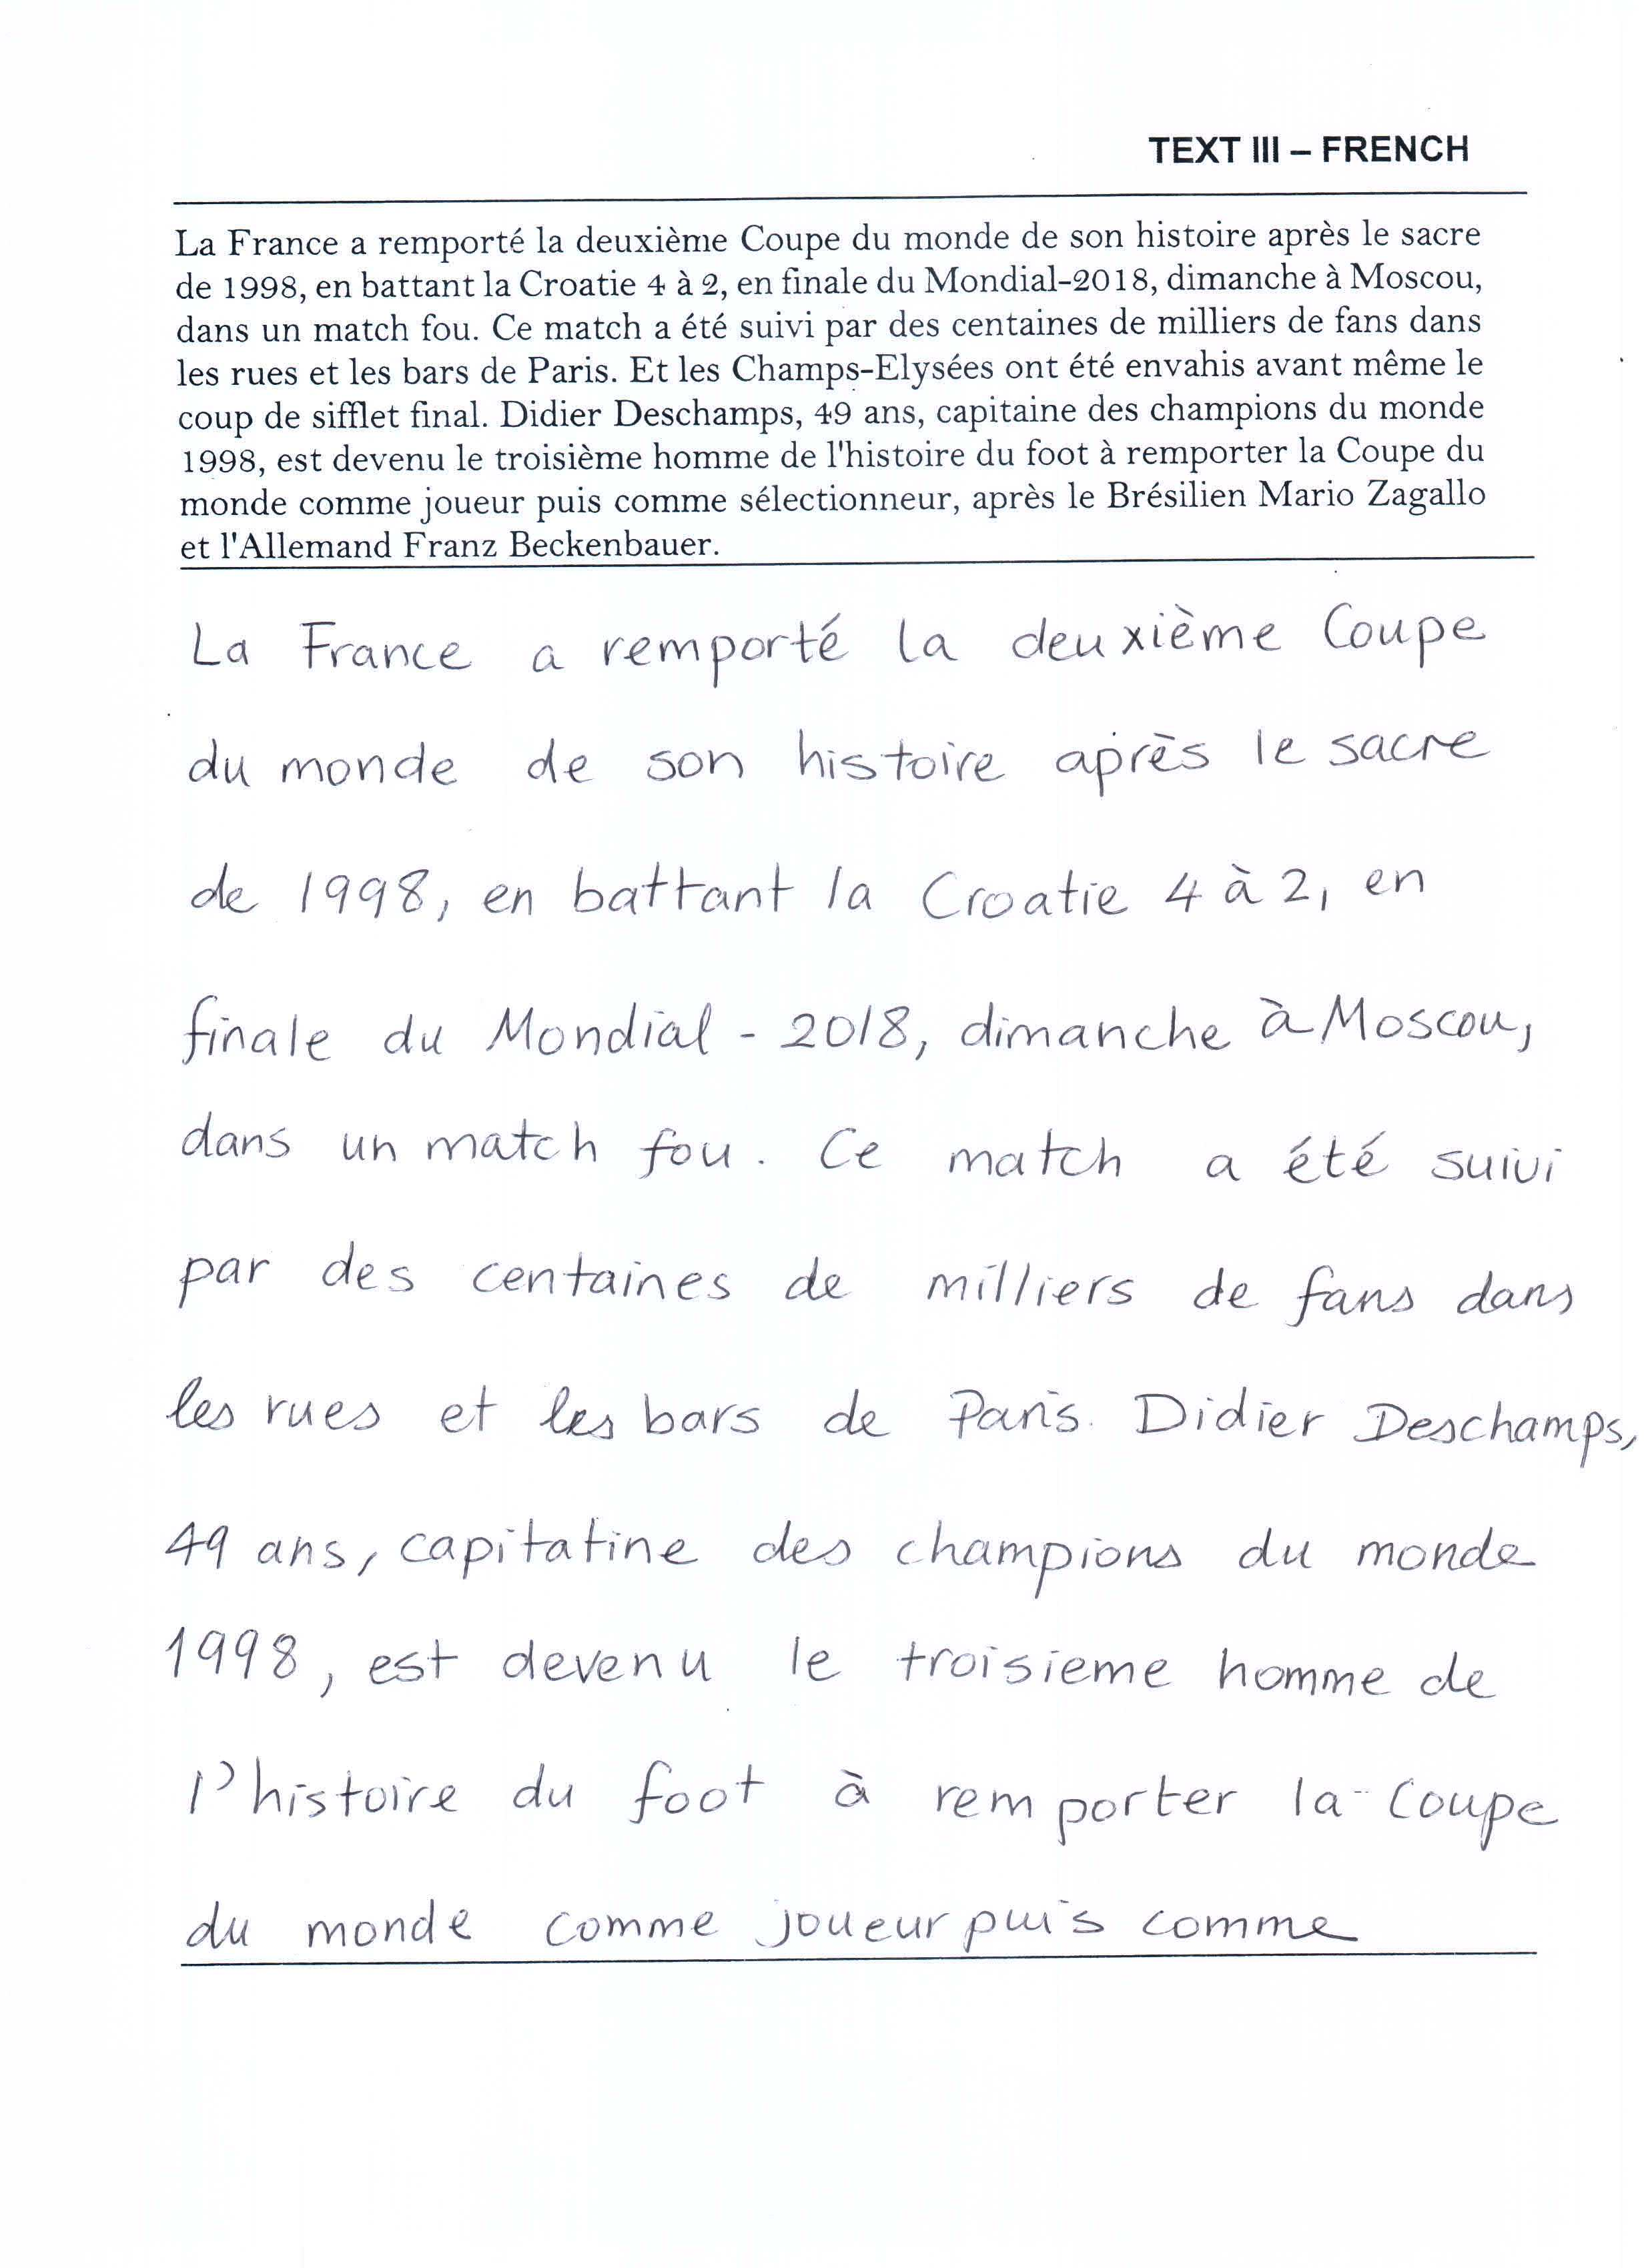
\includegraphics[width=0.4\textwidth]{images/5.jpeg}
    \caption{Image before clipping}
    \label{fig:clipping-example}
\end{figure}

\begin{figure}
    \centering
    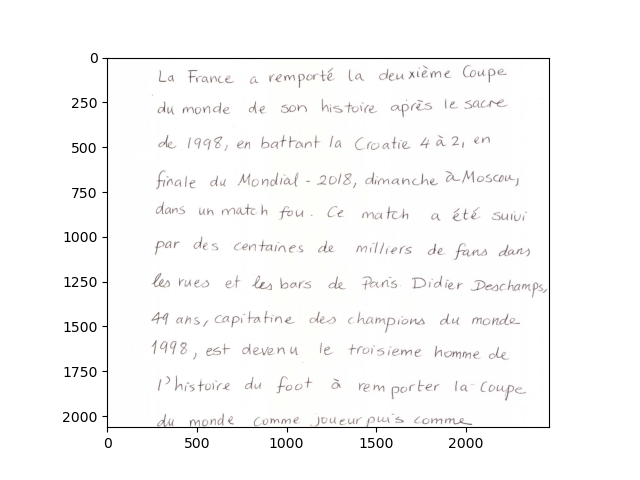
\includegraphics[width=0.4\textwidth]{images/img5_result.png}
    \caption{Image after clipping}
    \label{fig:clipping-result}
\end{figure}

\subsection{Line Segmentation}
As extracting features from lines is better than from the whole document, and classifying on each line helps to take a majority vote, We implemented a vectorized module to segment the document into lines using row histogram as shown in \ref{fig:histogram}. The docs are scanned vertically, so as shown in \ref{fig:bounding-boxes}, Detecting minima on a row histogram can get the boundaries to cut the lines on, as they are almost horizontal. We did not use the concept of local minima in Detecting peaks as there is a lot of local minima that are not considered as line boundaries. We considered that the line boundary exists when there is an abrupt change in the histogram that makes it jump over $1/5$ of its mean. Some lines can be splitted into two lines, one of them has a small height. This happens because of different hand-writings. To tackle this problem, we filtered all lines that have black-pixel count less than $1/6$ of the mean of this count on all extracted lines. 

\begin{figure}
    \centering
    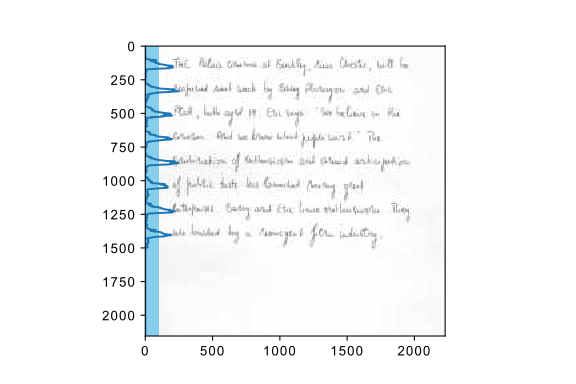
\includegraphics[width=0.5\textwidth]{images/histo.png}
    \caption{Row Histogram on Document to segment lines}
    \label{fig:histogram}
\end{figure}

\begin{figure}
    \centering
    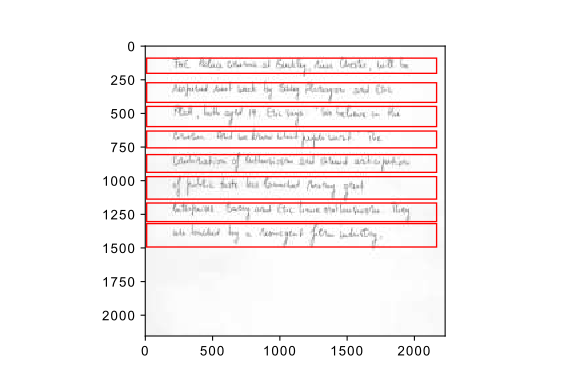
\includegraphics[width=0.5\textwidth]{images/BB.png}
    \caption{Resulting Bounding Boxes generated using Histogram}
    \label{fig:bounding-boxes}
\end{figure}



%%%%%%%%%%%%%%%%%%%%%%%%%%%%%%%%%%%%%%%%%%%%%%%%%%%%%%%%%%%%%%%%%%%%%%%%%%%%%%%%

\section{FEATURE EXTRACTION MODULE}
\begin{figure}[h!]
    \centering
    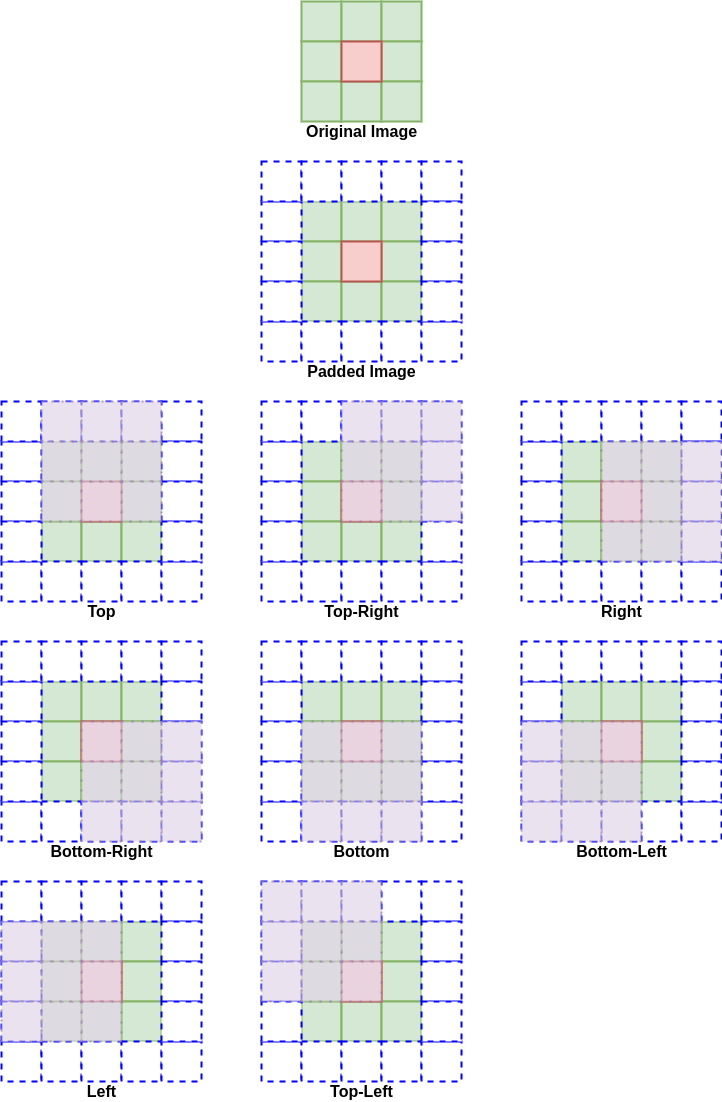
\includegraphics[width=0.4\textwidth]{images/lbp.png}
    \caption{Illustration of our vectorized implementation of LBP texture descriptor.}
    \label{fig:lbp-implementation}
\end{figure}

The feature extraction module includes \textbf{local binary pattern}\emph{(LBP)} texture descriptor. Other feature extractor were considered, as well. However, after many experiments, we found out \emph{LBP} texture descriptor performs the best in our case. The other feature extractors are discussed in later sections. Although \emph{LBP} features offer high accuracy, \textbf{skimage} implementation is not vectorized and heavily depends on \emph{loops}. The extraction of \emph{LBP} features for a single form can take up to $0.5$ second. That's why, we come up with a vectorized implementation that speeds up processing to up to $0.02$ second per form. \\

Figure \ref{fig:lbp-implementation} shows the \textbf{vectorized implementation} on a simple $3X3$ image matrix. The implementation goes as follows :
\begin{enumerate}
    \item The input image is \emph{padded} with \emph{zeros} from all directions with the \emph{LBP} radius size.
    \item An \emph{LBP} map with the same dimensions as the input image is initialized with zeros.
    \item The whole original image is displaced to the top and compared to the padded image. Using this method, we compare all pixels in parallel instead of looping over each pixel.
    \item The resultant map is, then, multiplied by $2$ raised to the power of \emph{number of iteration}, then added to the \emph{LBP} map. \textbf{Note that,} \emph{number of iteration} ranges from $0$ to $7$, as only $8$ directions are considered to speed up the implementation.
    \item Steps $3$ and $4$ are repeated for \emph{top-right}, \emph{right}, \emph{bottom-right}, \emph{bottom}, \emph{bottom-left}, \emph{left} and \emph{top-left} directions.
    \item A histogram is calculated for the output \emph{LBP} map with $256$ bins. The histogram is normalized by its mean, according to the original \emph{LBP} implementation.
\end{enumerate}

%%%%%%%%%%%%%%%%%%%%%%%%%%%%%%%%%%%%%%%%%%%%%%%%%%%%%%%%%%%%%%%%%%%%%%%%%%%%%%%%

\section{CLASSIFICATION MODULE}
For this work, $5$ classifiers are considered for experimentation, which are \textbf{Support Vector Machines} \emph{(SVM)}, \textbf{k-Nearest Neighbors} \emph{(KNN)}, \textbf{Random Forests} \emph{(RF)}, \textbf{Logistic Regression} \emph{(LR)} and \textbf{Naive Bayes} \emph{(NB)}. However, for our system, we choose \emph{SVM}, as it's the best performing classifier based on accuracy. At the same time, due to the small size of test cases, it is slightly slower than other classifiers like \emph{KNNs}, which can be acceptable. \\

The \emph{classification module} can have $3$ modes based on our implementation :
\begin{enumerate}
    \item \textbf{Complete train :} where the system is trained on complete data of authors with a specific number of forms. This is used as an initial experiment with the dataset and helped us determine the initial set of features.
    \item \textbf{Sampled train :} this mode mimics the test environment. It reads the whole dataset and generate a specific number of random test cases of $3$ writers, $2$ samples per writer and only $one$ test sample. This enables us to tune our parameters and choose our final techniques, which are, then, implemented and refined.
    \item \textbf{Test :} \emph{main pipeline} for the provided test environment, where the system takes the test directory and generates the output labels and time in text files.
\end{enumerate}


%%%%%%%%%%%%%%%%%%%%%%%%%%%%%%%%%%%%%%%%%%%%%%%%%%%%%%%%%%%%%%%%%%%%%%%%%%%%%%%%

\section{PERFORMANCE ANALYSIS}
\begin{table}[h!]
\centering
\begin{tabular}{||c | c | c||}
 \hline
 Classifier & 100 test samples & 1000 test samples \\ [0.5ex] 
 \hline\hline
 Support Vector Machine & 100\% & 99.7\% \\ 
 \hline
 k-Nearest Neighbors & 99\% & 99.4\% \\
 \hline
 Random Forest & 99\% & 99.6\% \\
 \hline
 Logistic Regression & 100\% & 99.5\% \\
 \hline
 Naive Bayes & 100\% & 98.9\% \\ [1ex] 
 \hline
\end{tabular}
\caption{Comparison between accuracies of different classifiers using LBP feature and different sample size.}
\label{table:1}
\end{table}

\begin{table}[h!]
\centering
\begin{tabular}{||c | c||}
 \hline
 Component & Execution Time \\ [0.5ex] 
 \hline\hline
 Form Clipping & 0.09 \\ 
 \hline
 Line Segmentation & 0.06 \\
 \hline
 LBP Features & 0.12 \\
 \hline
 Classifier Training & 0.01 \\
 \hline
 Complete Test Case & 2.00 \\ [1ex] 
 \hline
\end{tabular}
\caption{Average execution time of different system components (measured in seconds).}
\label{table:2}
\end{table}

\subsection{Accuracy Analysis}
As mentioned before, different approaches are considered for both feature extraction and classification. \\
We start by examining different feature extractors. According to \cite{c1}, the most promising texture descriptors are \emph{LBP}, \emph{LPQ} and \emph{GLCM}. We tried these texture descriptors, however we find that \emph{LBP} offers the most accurate and fast results, so we considered it for further experimentation. \emph{LBP} offers $99\%$ average accuracy with all classifiers in \textbf{sampled train mode}, however \emph{LPQ} and \emph{GLCM} offers around $88\%$ and $81\%$, respectively. \\
Regarding the classifiers, table \ref{table:1} shows the accuracy of different classifiers using \emph{LBP} features on $100$ and $1000$ random test cases. We can see that \emph{SVM} and \emph{RF} offer comparable results, however we choose \emph{SVM}, as it is more robust to \emph{preprocessor} failures and offers more consistent accuracy.

\subsection{Time Analysis}
We try to maintain our system accuracy within reasonable execution time. Different components are implemented and optimized for time. The execution times for different components are shown in table \ref{table:2}.


%%%%%%%%%%%%%%%%%%%%%%%%%%%%%%%%%%%%%%%%%%%%%%%%%%%%%%%%%%%%%%%%%%%%%%%%%%%%%%%%

\section{OTHER APPROACHES}
As mentioned before, we considered other different approaches in our experiments. In this section, we discuss, in some details, other considered approaches.

\subsection{Preprocessing}
We considered training the classifier on the whole form instead of separate lines, however this resulted in a huge performance impact, due to the small test cases. Moreover, we tried to segment out \textbf{connected components} from lines in the \emph{preprocessor}, in order to provide more training samples. Unfortunately, this does not work, as well, as the extracted features are not as good as that of complete lines. That's why, we decided to continue using separate lines in our system.

\subsection{Feature Extraction}
We, also, considered other feature extraction methods based on \emph{texture descriptors}, including :
\begin{itemize}
    \item \textbf{Local Phase Quantization (LPQ) :} offers around $95\%$ accuracy on randomly-sampled test cases, which is worse than \emph{LBP}. This is mainly because the form images do not contain heavy blurring and scanning issues.
    \item \textbf{Gray Level Co-occurrence Matrix (GLCM) :} very primitive texture descriptor, offers humble performance.
    \item \textbf{CSLBCoP :} integrates \emph{GLCM} with \textbf{Center Symmetric Local Binary Pattern} \emph{(CSLBP)} of an image to obtain the feature pattern. It offers even lower performance than \emph{LPQ} with around $90\%$ on randomly-sampled test cases.
    \item \textbf{Principal Component Analysis (PCA) :} we tried extracting principal components from \emph{LBP} features, in order to reduce the feature vector size and avoid overfitting. Unfortunately, this does not improve performance over complete \emph{LBP} features.
\end{itemize}

\subsection{Classification}
As mentioned before, other classifiers are considered as well. However, based on the previous analysis, we choose \emph{SVM} as our best classifier. We use \textbf{sklearn} for training all mentioned classifiers. Also, we use \textbf{sklearn grid search} for model parameters tuning.


%%%%%%%%%%%%%%%%%%%%%%%%%%%%%%%%%%%%%%%%%%%%%%%%%%%%%%%%%%%%%%%%%%%%%%%%%%%%%%%%

\section{WORKLOAD DISTRIBUTION}
\begin{center}
\begin{tabular}{||c |c ||} 
 \hline
 Name & Workload \\ [0.5ex] 
 \hline\hline
  Mohamed Shawky Zaky & \\
 \hline
 Remonda Talaat Eskarous &  \\
  \hline
 Mohamed Ahmed Mohamed Ahmed & \\
 \hline
 Mohamed Ramzy Helmy & \\ [1ex] 
 \hline
\end{tabular}
\end{center}

%%%%%%%%%%%%%%%%%%%%%%%%%%%%%%%%%%%%%%%%%%%%%%%%%%%%%%%%%%%%%%%%%%%%%%%%%%%%%%%%

\section{CONCLUSION AND FUTURE WORK}
\emph{Classical approaches} can be used to build a very robust writer identification system. In this work, we adopt different \emph{texture descriptors} as feature extractors. We show that \emph{LBP} features are simple yet powerful feature extractor for handwriting encoding. Also, we discuss the performance of different classifiers and illustrate that \emph{SVM} offers the best consistent performance. We, also, introduced the idea of dividing the form into lines and taking the majority vote, which greatly improves the performance in our test environment, because of small test cases. \\
This work can be improved in the following ways :
\begin{enumerate}
    \item Improve \emph{preprocessor} to handle different illuminations and perform color correction.
    \item Expand \emph{LBP} features to include more than $8$ neighbors.
    \item Try to ensemble multiple classifiers output for better and more stable performance.
\end{enumerate}


%%%%%%%%%%%%%%%%%%%%%%%%%%%%%%%%%%%%%%%%%%%%%%%%%%%%%%%%%%%%%%%%%%%%%%%%%%%%%%%%

\begin{thebibliography}{99}
\bibitem{c1} Writer identification using texture features: A comparative study.
\bibitem{c2} Text independent writer recognition using redundant writing patterns with contour-based orientation and curvature features.
\bibitem{c3} An improved online writer identification framework using codebook descriptors.
\end{thebibliography}

%%%%%%%%%%%%%%%%%%%%%%%%%%%%%%%%%%%%%%%%%%%%%%%%%%%%%%%%%%%%%%%%%%%%%%%%%%%%%%%%

\end{document}
